\documentclass{article}
\usepackage{enumitem}
\usepackage{listings}
\usepackage{amsfonts}
\usepackage{latexsym}
\usepackage{fullpage}
\usepackage{graphicx}
\usepackage{paralist}
\usepackage{tikz-timing}

\lstdefinelanguage{VHDL}{
  morekeywords={
    library,use,all,ENTITY,IS,PORT,IN,OUT,end,architecture,of,
    begin,and, ARCHITECTURE, IF, THEN, SIGNAL,END, PROCESS
  },
  morecomment=[l]--
}

\usepackage{xcolor}
\colorlet{keyword}{blue!100!black!80}
\colorlet{comment}{green!90!black!90}
\lstdefinestyle{vhdl}{
  language     = VHDL,
  basicstyle   = \ttfamily\scriptsize,
  keywordstyle = \color{keyword}\bfseries\ttfamily,
  commentstyle = \color{comment}\ttfamily,	
  tabsize=1
}

\renewcommand{\lstlistingname}{Code}

% Default margins are too wide all the way around. I reset them here
\setlength{\topmargin}{-.5in}
\setlength{\textheight}{9in}
\setlength{\oddsidemargin}{.125in}
\setlength{\textwidth}{6.25in}


%\let\oldenumerate\enumerate
%\renewcommand{\enumerate}{
  %\oldenumerate
  %\setlength{\itemsep}{1pt}
  %\setlength{\parskip}{0pt}
  %\setlength{\parsep}{0pt}
%}


\begin{document}
\title{Organization of Digital Computer Lab \\ EECS112L/CSE 132L}
\author{\textbf{Assignment 4 }\\ \textbf{Pipeline MIPS} \\ \\
prepared by: Team Stressed \\ Student name: \\ Mansi Tyagi \\ Student ID: \\23334840\\ \\ Student name: \\ Erik Henriquez\\ Student ID: \\57374677\\ \\ Student name: \\ Kevin Chau \\ Student ID: \\76934313\\ \\ Student name: \\ Steven Chow\\Student ID: \\70916812\\ \\ Student name: \\ Paul Dao \\Student ID: \\30658761\\ \\
EECS Department\\ Henry Samueli School of Engineering \\ University of California, Irvine \\ \\
{March 13, 2016}} 


\date{}
\maketitle


\section{Summary of Processor Design}
\subsection{What We Learned}
In this part of the assignment, we used our datapath from Lab 3, which implemented a complete single-cycle processor, and converted it into a pipelined processor. The processor we created pipelines the datapath and is capable of stalling and forwarding, and is capable of evaluating R, I, and J-Type instructions. In addition to simulating the processor, we also needed to synthesize it. We used Synopsis to determine the power consumption, area requirements, and clock frequency necessary to build our processor design. Although the use of Synopsis was initially very troublesome, we appreciated the fact that we were able to use tools that well-known corporations, like Intel and AMD, use to design and fabricate their own products.

\subsection{Description}
For our pipelined processor, we implemented all the components that we created for our single-cycle processor in lab 3. In order to create a pipelined processor, we created arrays which would function as the pipeline registers that are present between each stage. These registers are controlled by the rising clock edge. In each cycle, every stage would compute its instructions by using the values the components would receive from the pipeline register preceeding it. Since the registers are controlled by the rising clock edge, the previous values would be rewritten by the new ones, advancing each instruction by a stage each cycle.  In addition to those, we also created a Hazard and Forwarding unit. The Hazarding unit detected when a load, structural, or control hazard were present. If they were, it would act accordingly to stall the next instruction as needed. The Forwarding unit detected when forwarding was necessary. If it was, it would forward the data to the necessary proceeding instructions. We also needed to add a comparator outside of the ALU and in the ID stage to reduce stalls when branches were taken. To control the comparator, we needed to incorporate two muxes to choose two of the four possible inputs. We also needed to include two more 3-to-1 muxes before the ALU to control when information needs to be forwarded to later instructions. //TO DO: ADD MORE ABOUT MODIFICATIONS FOR SYNTHESIS \\

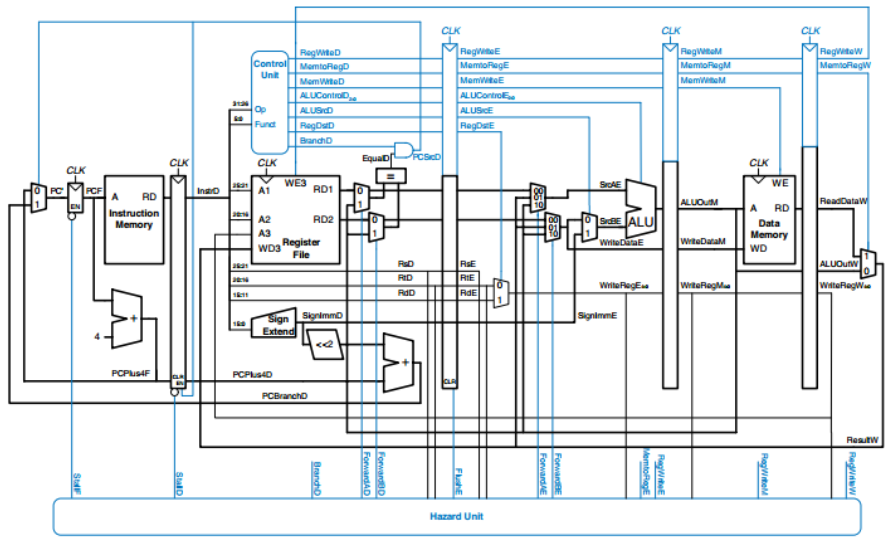
\includegraphics[width=0.8\textwidth]{PipelinedDatapath.png} \\ \\


\subsection{Testbench Architecture}
Our testbench is the same as the one we used for Lab 3. We needed to add more cycles to accomodate the different cycles, since each instruction will now take 5 cycles, one for each stage, instead of one.


\section{Sample Program}
\subsection{Instructions}
We were given a list of 18 32-bit MIPS instructions, written in hexadecimal form. Before proceeding, we decoded these instructions into a human-readable format.

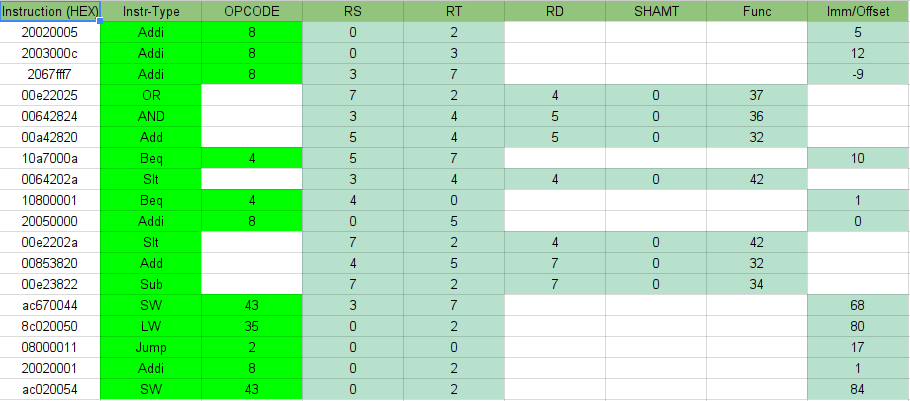
\includegraphics[width=0.8\textwidth]{example_program_decoded_instructions.png}

After decoding the instructions, we worked out the theoretical state of the Register File after every instruction. Of the two branch instructions in our sample program, one is successful and results in four instructions being skipped. There is also a jump instruction near the end of the program, which skips the final two instructions and moves the program counter into undefined memory, resulting in a "garbage" instruction. \\


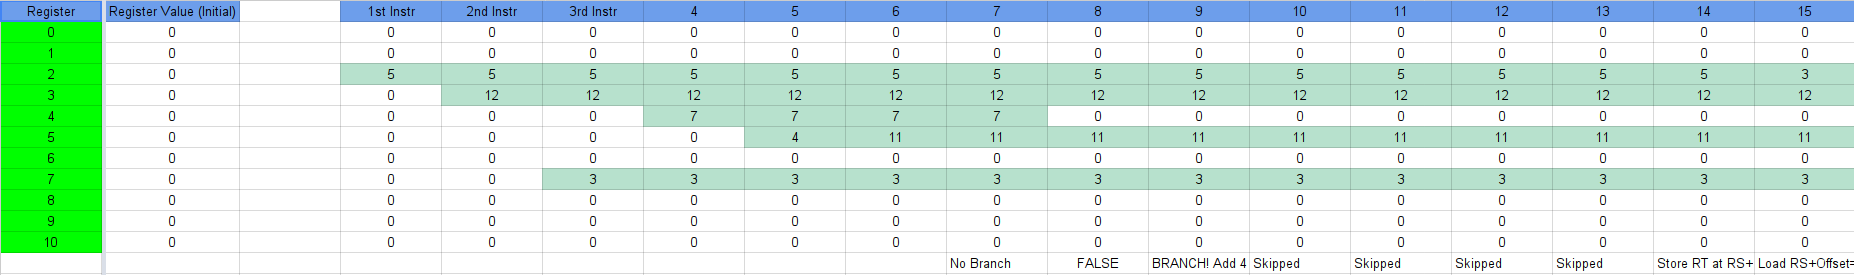
\includegraphics[width=0.8\textwidth]{example_program_registerfile_part1.png} \\ \\
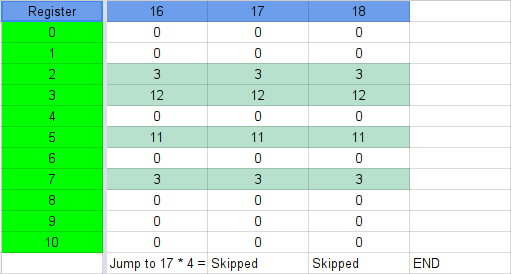
\includegraphics[width=0.25\textwidth]{example_program_registerfile_part2.png} 
	
\subsection{Simulation Waveform}
\bfseries{After designing and testing our Processor, we generated the following waveforms:} \\ \\

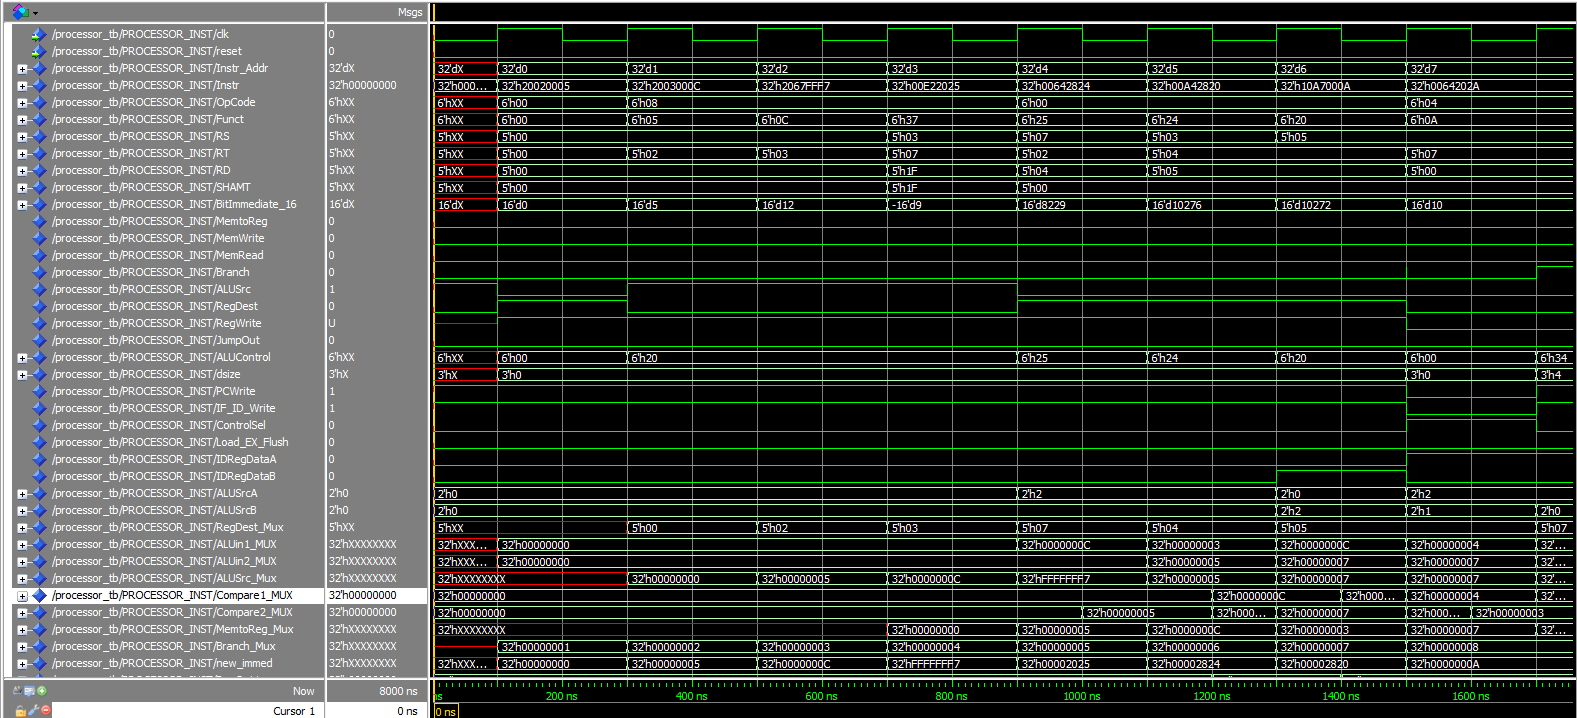
\includegraphics[width=0.8\textwidth]{Waveform1.png} \\ \\
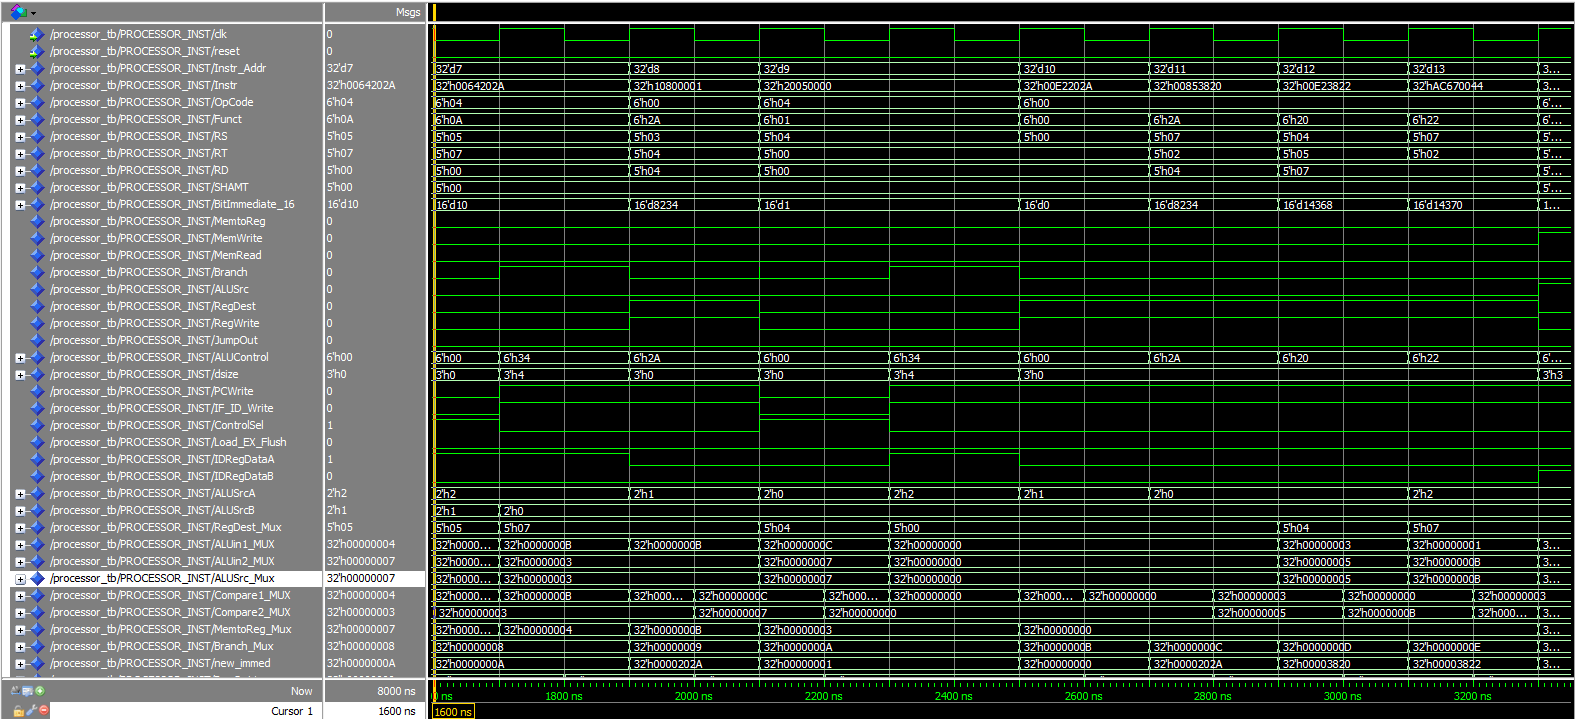
\includegraphics[width=0.8\textwidth]{Waveform2.png} \\ \\
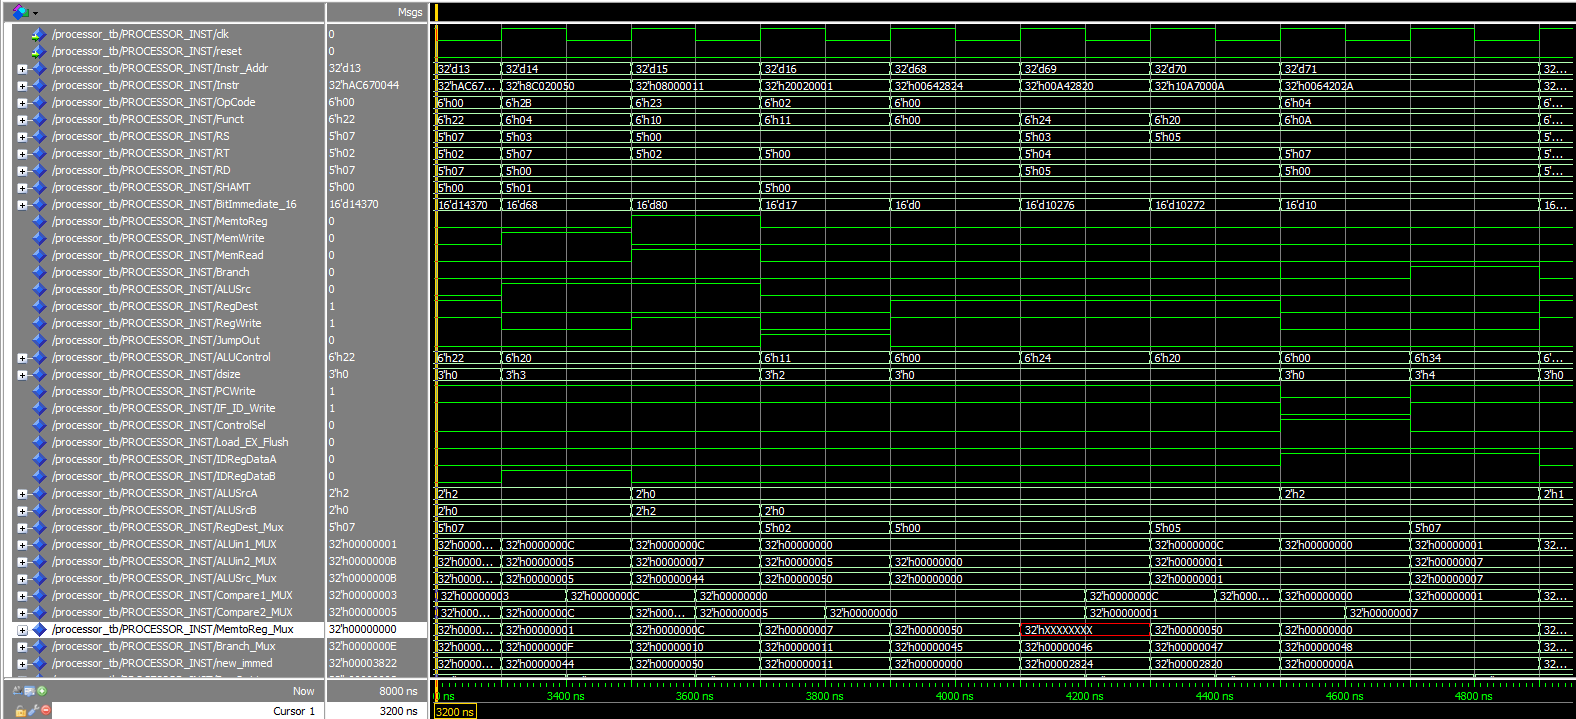
\includegraphics[width=0.8\textwidth]{Waveform3.png} \\

Each of the pipeline stages, hazards, forwarding, and stalls were correctly implemented. The instruction values shown in each cycle correlate to the instruction in the ID stage, while other various signals indicate the values for other instructions in different stages; for example, ALUresult outputs the evaluated ALU value from the EX stage. The pipeline registers indicate the transition of each instruction into the next stage.

\section{Synthesis}
Through synthesis, we were able to determine the power consumption, area requirements, and frequency of our processor design. Synopsis, a software suite provided by our university, was used to perform synthesis on our design. After adjusting the analysis, elaboration, and synthesis files and scripts, we synthesized our processor design and successfully generated various reports on our processor's performance. // TO DO: FIX THIS STUFF

\subsection{Power Consumption}
Our processor's total power consumption came out to 20.3 mW. From the power hierarchy we generated, approximately 74\% of the power consumption is due to our register file component, with another 19.9\% being used by the ALU. All other components use three orders of magnitude less power.

\subsection{Area}
After reading the generated area reports, we could not determine the units being used in the report. However, Synopsys reported that our Design area would be 82228.100300, with a Combinational Area of approximately 16868. We achieved these results using Professor Yaghini's SRAM. However, when using our Data Memory component (written in VHDL), our Combinational Area was over twice as large.

\subsection{Required Frequency}
According to the generated timing report, our Critical Path Length was 3.18 ns. In order to accommodate this and eliminate negative slack, we raised our clock period from 2.0 ns to 3.2 ns. This results in a frequency of approximately 312.5 MHz.

The majority of our timing delay comes from our PC adder, accounting for approximately 2.25 ns of the critical path length. We expect to see a reduction in the critical path in future labs, where our Adder components will not be required.

\section{Known Issues} 
Due to our unfamiliarity with SystemVerilog, we chose not to use the testbench to preload instruction memory. For the Questasim simulation, we read the example program instructions from a file.  For synthesis, we created a second version of instruction memory that has instructions preloaded into memory in order to synthesize the Processor properly.
\\
\section{Conclusion}

As a complete single-cycle processor, our project now supports a larger subset of the full MIPS instruction set. It is capable of all three types of MIPS instructions: R-type, I-type, and J-type. Through synthesis, we were able to determine the area, power and frequency properties our processor design would have if fabricated. Finally, with this complete processor, we should be well prepared to implement pipelining in our future assignment. //TO DO: WRITE...


\end{document}
